%%%%%%%%%%%%%%% Use cases %%%%%%%%%%%%%%%%%%%%%%%%%

\section{Use cases}
\label{sec:use-cases}

In this section we will state the main use cases identified and we detail the
interactions of the main scenarios for each of them.

%%%%%%%%%%%%%%% Repository Management %%%%%%%%%%%%%%%%%%%%%%%%%

\subsection{Repository management}
\label{subsec:rm-use-cases}
The Figure \ref{img:uc-repository} shows the main use cases related with the
repository management process, which are detailed in Tables
\ref{table:browse-app}, \ref{table:share-app} and \ref{table:retrieve-app}.

\begin{figure}[h!]
 \begin{center}
 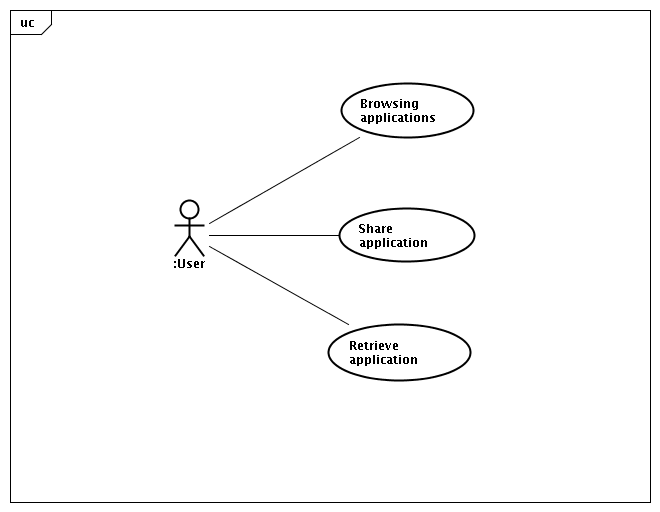
\includegraphics[scale=0.5]{diagrams/UseCasesDiagram-sharing.png}
  \caption{\label{img:uc-repository}Repository management use cases}
 \end{center}
\end{figure}


%%Browse applications
\begin{table}[h!]
	\small
    \begin{center}
		\begin{tabular}{||r|l||}
		\hline \hline
		\multicolumn{2}{||c||}{\bfseries{Browse applications}} \\
		\hline
		\hline 
		Brief description: & Actor browses repository applications. \\
		\hline
		Actors: & Authenticated ASTRA user. \\
		\hline
		Preconditions: &  There are applications visible for that user. \\
		\hline \hline
		\multicolumn{2}{||l||}{Basic flow of events:} \\
		\hline \hline
			1. & User expands the applications tree. \\
			2. & User selects an application. \\
			3. & System retrieves all the information related to it.	\\ 
			4. & System displays the information. \\ \hline \hline
		Postconditions: &  - \\
		\hline \hline
		\end{tabular}
		\caption{\label{table:browse-app} Browse applications - general scenario
		description}
	\end{center}
\end{table}

%%Share application
\begin{table}[h!]
	\small
    \begin{center}
		\begin{tabular}{||r|l||}
		\hline \hline
		\multicolumn{2}{||c||}{\bfseries{Share application}} \\
		\hline
		\hline 
		Brief description: & Actor shares an application in the repository. \\
		\hline
		Actors: & Authenticated ASTRA user. \\
		\hline
		Preconditions: &  A local application has been selected. \\
		\hline \hline
		\multicolumn{2}{||l||}{Basic flow of events:} \\
		\hline \hline
			1. & User selects share application. \\
			2. & System displays all the information related to it. \\
			3. & User customizes the parameters to be shared: \\ 
			   & visibility in terms of communities, rules, description, etc.	\\ 
			4. & User confirms the sharing process. \\ 
			5. & System validates the parameters. \\
			6. & System confirms the application was shared properly. \\\hline \hline
		Postconditions: &  A new application is available in the repository. \\
		\hline \hline
		\end{tabular}
		\caption{\label{table:share-app} Share application - general scenario
		description}
	\end{center}
\end{table}

%%Retrieve application
\begin{table}[h!]
	\small
    \begin{center}
		\begin{tabular}{||r|l||}
		\hline \hline
		\multicolumn{2}{||c||}{\bfseries{Retrieve application}} \\
		\hline
		\hline 
		Brief description: & Actor retrieves an application from the repository. \\
		\hline
		Actors: & Authenticated ASTRA user. \\
		\hline
		Preconditions: &  An application from the repository has been selected. \\
		\hline \hline
		\multicolumn{2}{||l||}{Basic flow of events:} \\
		\hline \hline
			1. & User selects retrieve application. \\
			2. & System displays all the information related to it. \\
			3. & User customizes the parameters to be retrieved: rules and description.	\\ 
			4. & User confirms the retrieving process. \\ 
			5. & System validates the parameters. \\
			6. & System confirms the application was retrieved properly. \\\hline \hline
		Postconditions: &  A new application is available in the user local space. \\
		\hline \hline
		\end{tabular}
		\caption{\label{table:retrieve-app} Retrieve application - general scenario
		description}
	\end{center}
\end{table}


%%%%%%%%%%%%%%% Searching %%%%%%%%%%%%%%%%%%%%%%%%%
\clearpage

\subsection{Searching}
\label{subsec:searching-use-cases}
The Figure \ref{img:uc-searching} shows the main use cases related with the
searching requirements, which are detailed in Tables
\ref{table:search-criteria} and \ref{table:search-similarity}.

\begin{figure}[h!]
 \begin{center}
 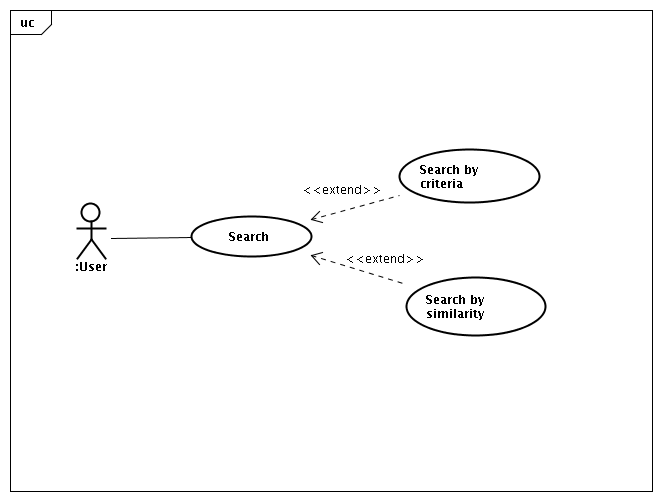
\includegraphics[scale=0.5]{diagrams/UseCasesDiagram-searching.png}
 \end{center}
 \caption{\label{img:uc-searching}Searching use cases}
\end{figure}

%%Search by criteria
\begin{table}[h!]
	\small
    \begin{center}
		\begin{tabular}{||r|l||}
		\hline \hline
		\multicolumn{2}{||c||}{\bfseries{Searching by criteria}} \\
		\hline
		\hline 
		Brief description: & Actor searches for an application typing some keywords
		and a criterion.\\
		\hline
		Actors: & Authenticated ASTRA user. \\
		\hline
		Preconditions: &  - \\
		\hline \hline
		\multicolumn{2}{||l||}{Basic flow of events:} \\
		\hline \hline
			1. & User enters one or more keywords. \\
			2. & User selects a criterion (by tags, by description, by type or any). \\
			3. & System performs a search based on the given parameters. \\
			4. & System displays matching applications.\\ 
		\hline \hline
		Postconditions: &  - \\
		\hline \hline
		\end{tabular}
		\caption{\label{table:search-criteria}Search by criteria - general scenario
		description}
	\end{center}
\end{table}

%%Search by similarity
\begin{table}[h!]
	\small
    \begin{center}
		\begin{tabular}{||r|l||}
		\hline \hline
		\multicolumn{2}{||c||}{\bfseries{Searching by similarity}} \\
		\hline
		\hline 
		Brief description: & Actor searches for applications that are similar to a
		given application.\\
		\hline
		Actors: & Authenticated ASTRA user. \\
		\hline
		Preconditions: &  - \\
		\hline \hline
		\multicolumn{2}{||l||}{Basic flow of events:} \\
		\hline \hline
			1. & User selects an application. \\
			2. & System compares the selected application with \\ 
			  & applications in the repository using different measures. \\ 
			3. & System displays matching applications.\\ 
		\hline \hline
		Postconditions: &  - \\
		\hline \hline
		\end{tabular}
		\caption{\label{table:search-similarity}Search by similarity - general
		scenario description}
	\end{center}
\end{table}



%%%%%%%%%%%%%%% Tags management %%%%%%%%%%%%%%%%%%%%%%%%%
\clearpage

\subsection{Tags management}
\label{subsec:tags-use-cases}

The Figure \ref{img:uc-tagging} shows the main use cases related with the
tags management process, which are detailed in Tables \ref{table:add-tag}
and \ref{table:remove-tag}.

\begin{figure}[h!]
 \begin{center}
 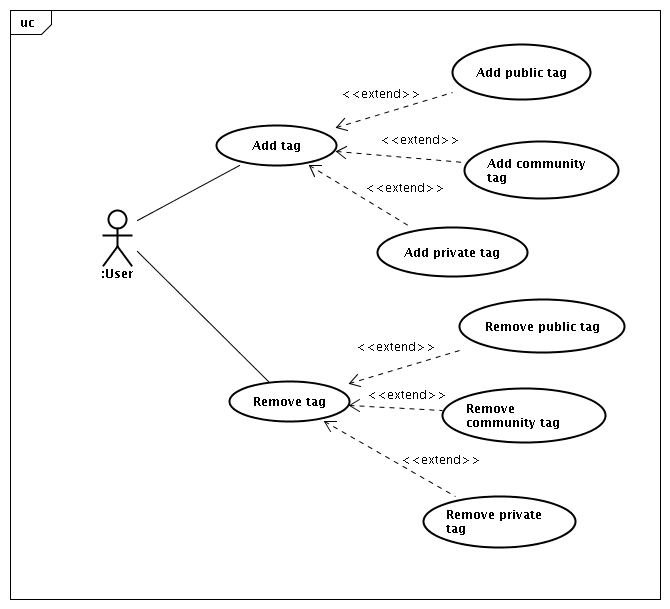
\includegraphics[scale=0.5]{diagrams/UseCasesDiagram-tagging.png}
 \end{center}
 \caption{\label{img:uc-tagging}Tagging use cases}
\end{figure}


%%Add tag
\begin{table}[h!]
	\small
    \begin{center}
		\begin{tabular}{||r|l||}
		\hline \hline
		\multicolumn{2}{||c||}{\bfseries{Add tag}} \\
		\hline
		\hline 
		Brief description: & Actor adds a tag to an application specifying the level\\
		& of visibility of the tag. \\
		\hline
		Actors: & Authenticated ASTRA user. \\
		\hline
		Preconditions: & An application has been selected. \\
		\hline \hline
		\multicolumn{2}{||l||}{Basic flow of events:} \\
		\hline \hline
			1. & User enters a tag name. \\
			2. & User specifies tag visibility. \\
			3. & System validates tag. \\
			4. & System stores the tag. \\ 
			5. & System confirms that tag has been added. \\
		\hline \hline
		Postconditions: & A new tag is associated to the application \\
		&  and is made available within the proper scope. \\
		\hline \hline
		\end{tabular}
		\caption{\label{table:add-tag} Add tag - general scenario description}
	\end{center}
\end{table}

%%Remove tag
\begin{table}[h!]
	\small
    \begin{center}
		\begin{tabular}{||r|l||}
		\hline \hline
		\multicolumn{2}{||c||}{\bfseries{Remove tag}} \\
		\hline
		\hline 
		Brief description: & Actor removes a tag from an application. \\
		\hline
		Actors: & Authenticated ASTRA user. \\
		\hline
		Preconditions: & User has previously tagged the selected application. \\
		\hline \hline
		\multicolumn{2}{||l||}{Basic flow of events:} \\
		\hline \hline
			1. & User selects a tag. \\
			2. & System displays option to remove the tag. \\
			3. & User chooses to remove the tag. \\
			4. & System deletes the tag.\\ 
			5. & System confirms that tag has been deleted. \\
		\hline \hline
		Postconditions: & The specified tag is no longer associated with the
		specified application. \\ \hline \hline
		\end{tabular}
		\caption{\label{table:remove-tag}Remove tag - general scenario description}
	\end{center}
\end{table}

%%%%%%%%%%%%%%% Others %%%%%%%%%%%%%%%%%%%%%%%%%
\clearpage

\subsection{Other general functionalities}
\label{subsec:others-use-cases}
The Figure \ref{img:uc-others} shows use cases that capture other general
functionalities, which are detailed in Tables \ref{table:login}, 
\ref{table:logout} and \ref{table:help}.

\begin{figure}[h!]
 \begin{center}
 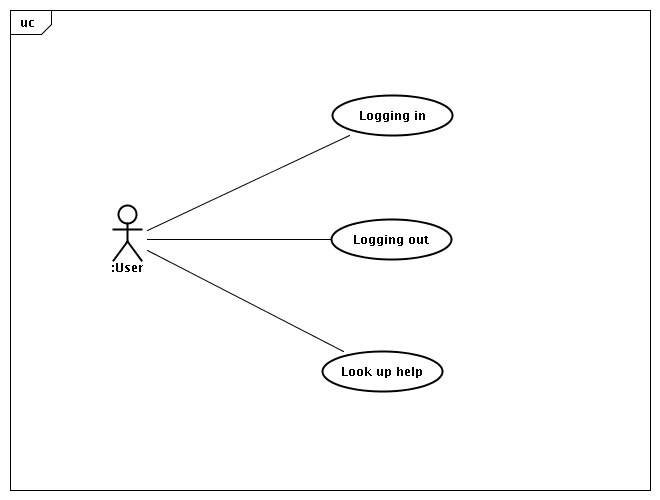
\includegraphics[scale=0.5]{diagrams/UseCasesOthers.png}
 \end{center}
 \caption{\label{img:uc-others}Other general functionalities}
\end{figure}

%%Logging in
\begin{table}[h!]
	\small
    \begin{center}
		\begin{tabular}{||r|l||}
		\hline \hline
		\multicolumn{2}{||c||}{\bfseries{Logging in}} \\
		\hline
		\hline 
		Brief description: & Actor logs in the system.\\
		\hline
		Actors: & Non-authenticated ASTRA user. \\
		\hline
		Preconditions: &  Login window is displayed. \\
		\hline \hline
		\multicolumn{2}{||l||}{Basic flow of events:} \\
		\hline \hline
			1. & User types username and password. \\
			2. & System validates them. \\
			3. & System loads user's profile. \\ 
			4. & System displays the main menu and disposes the login window. \\
			\hline \hline Postconditions: &  - \\
		\hline \hline
		\end{tabular}
		\caption{\label{table:login}Logging in - general scenario  description}
	\end{center}
\end{table}

%%Logging out
\begin{table}[h!]
	\small
    \begin{center}
		\begin{tabular}{||r|l||}
		\hline \hline
		\multicolumn{2}{||c||}{\bfseries{Logging out}} \\
		\hline
		\hline 
		Brief description: & Actor logs out of the system. \\
		\hline
		Actors: & Authenticated ASTRA user. \\
		\hline
		Preconditions: &  Main window is displayed. \\
		\hline \hline
		\multicolumn{2}{||l||}{Basic flow of events:} \\
		\hline \hline
			1. & User selects logout option. \\
			2. & System asks for confirmation. \\
			3. & User confirms. \\ 
			4. & System closes user's session, disposes the main window and \\
			   & displays the login window \\ 
		\hline \hline Postconditions: &  - \\
		\hline \hline
		\end{tabular}
		\caption{\label{table:logout}Logging out - general scenario description}
	\end{center}
\end{table}

%%Lookup help
\begin{table}[h!]
	\small
    \begin{center}
		\begin{tabular}{||r|l||}
		\hline \hline
		\multicolumn{2}{||c||}{\bfseries{Look up help}} \\
		\hline
		\hline 
		Brief description: & Actor looks up the online help. \\
		\hline
		Actors: & Authenticated ASTRA user. \\
		\hline
		Preconditions: &  -  \\
		\hline \hline
		\multicolumn{2}{||l||}{Basic flow of events:} \\
		\hline \hline
			1. & User selects online help option. \\
			2. & System retrieves the remote help. \\
			3. & System displays the help contents in an intuitive way. \\ 
			\hline \hline
		Postconditions: &  - \\
		\hline \hline
		\end{tabular}
		\caption{\label{table:help}Look up help - general scenario description}
	\end{center}
\end{table}